\subsection{Критическая интенсивность}

        Критической интенсивностью называется такое значение интенсивности, при котором траектории могут выходить за границы аттрактора и сваливаться в ноль.

        Например, на рисунке \ref{critical_intensity_beta_noise} изображен график критической интенсивности для \(\beta\)-шума. Красным показана критическая интенсивность для границ доверительных интервалов, которые лежат ниже устойчивого равновесия. Синим - для границ, которые выше устойчивого равновесия. 

        \comment{Наверное, не понятно про какие границы доверительного интервала идет речь}

        \comment{Для 4-цикла сделать шаг меньше и подойти ближе к 2-циклу. Холмик должен получится}

        \begin{figure}
            \centering
            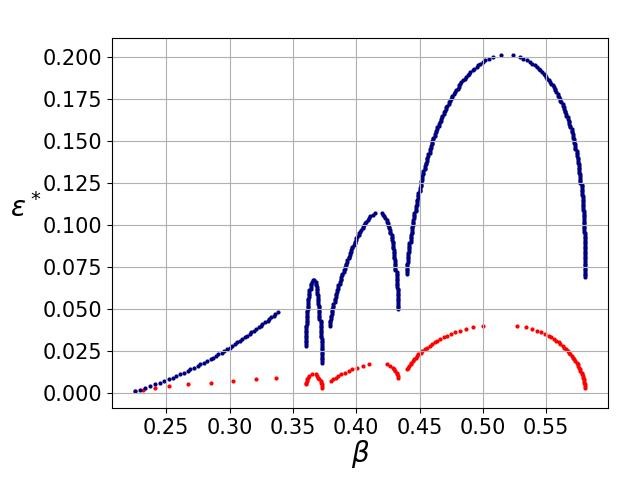
\includegraphics[width=\textwidth]{stochastic/critical_intensity_beta_noise.jpg}
        
            \captionsetup{justification=centering}
            \caption{}
            \label{critical_intensity_beta_noise}
        \end{figure}
        
        Обозначения аналогичны для графиков \(\alpha\)-шума (\ref{critical_intensity_alpha_noise}) и аддитивного шума (\ref{critical_intensity_additive_noise}).

        Интересно заметить, что в случае \(\alpha\)-шума и \(\beta\)-шума силуэты графиков очень похожи.

        \begin{figure}
            \centering
            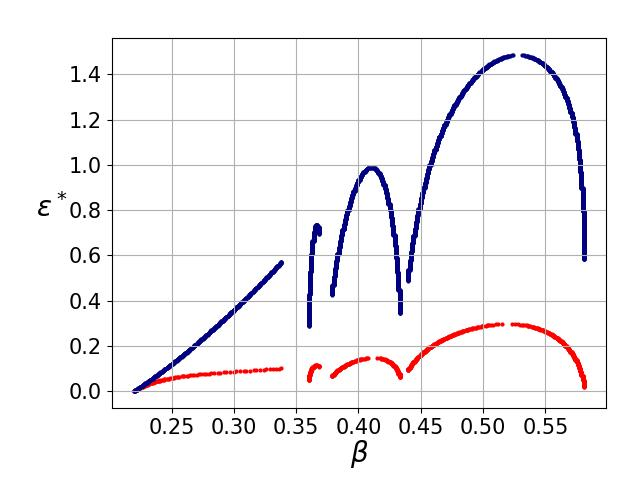
\includegraphics[width=\textwidth]{stochastic/critical_intensity_alpha_noise.jpg}
        
            \captionsetup{justification=centering}
            \caption{}
            \label{critical_intensity_alpha_noise}
        \end{figure}

        \begin{figure}
            \centering
            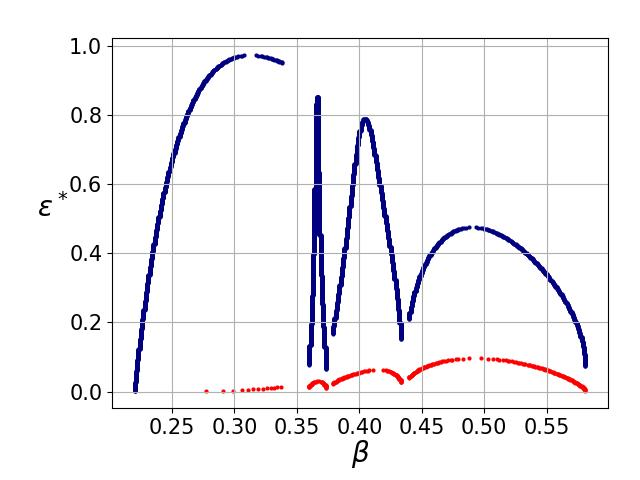
\includegraphics[width=\textwidth]{stochastic/critical_intensity_additive_noise.jpg}
        
            \captionsetup{justification=centering}
            \caption{}
            \label{critical_intensity_additive_noise}
        \end{figure}

        \comment{"Маловато будет!"}